% Draft for the Solar Filament Segmentation Challenge 2026 technical report (4 pages).
% Layout approximates the IEEE conference template (10 pt, two columns, US letter) so the page count
% is realistic; move the text into the official Overleaf template before submitting.
\documentclass[10pt,twocolumn,letterpaper]{article}
\usepackage[letterpaper,top=0.75in,bottom=1in,left=0.625in,right=0.625in,columnsep=0.25in]{geometry}
\usepackage{mathptmx}
\usepackage[T1]{fontenc}
\usepackage{graphicx,booktabs,amsmath,cite,balance}
\usepackage[hidelinks]{hyperref}
\usepackage[font=small,labelfont=bf,skip=3pt]{caption}
\setlength{\textfloatsep}{8pt plus 2pt}
\setlength{\floatsep}{6pt plus 2pt}
\setlength{\abovedisplayskip}{3pt}\setlength{\belowdisplayskip}{3pt}
\makeatletter
\renewcommand{\section}{\@ifstar{\fil@sec}{\fil@sec}}
\newcommand{\fil@sec}[1]{\par\smallskip\noindent{\normalsize\bfseries\MakeUppercase{#1}}\par\smallskip}
\makeatother
\renewcommand{\subsection}[1]{\par\smallskip\noindent{\itshape #1.}\ }
\pagestyle{empty}

\title{\Large\bfseries Whole-Disk U-Net Ensembles with PQ-Tuned Post-Processing\\for Solar Filament Segmentation}
\author{Johnson Chishimba\\{\small Affiliation, City, Country \quad email@example.com}}
\date{}

\begin{document}
\maketitle
\thispagestyle{empty}

\noindent{\small\bfseries\itshape Abstract---}{\small\bfseries We segment individual solar filaments in full-disk GONG H$\alpha$ observations for the Solar Filament
Segmentation Challenge 2026. The MAGFiLO training labels are noisy: 42\% of images were labelled by two or
three people, who agree with each other at a Panoptic Quality (PQ) of only 0.34. We therefore train a U-Net
on the \emph{average} of each image's annotators, segment the whole disk at 1024\,px in one pass, average five
fold models with test-time augmentation, and form instances with a post-processing step whose five settings
are tuned for PQ on out-of-fold predictions of all 707 training images. Out of fold, the method reaches
PQ 0.408 against each annotator (0.353 when all annotators of an image are pooled) and scores 0.36 on the
public leaderboard. Ablations show that a larger encoder, model averaging, a learned instance score and
ensemble calibration each change PQ by less than 0.005, and an error analysis attributes most of the
remaining loss to 1--2\,px boundary disagreement that annotators share.}\par\medskip

\section{Introduction}
Filaments are clouds of cool plasma suspended above magnetic polarity inversion lines; their eruptions drive
coronal mass ejections, so a reliable automatic detector matters for space-weather monitoring. The challenge
asks for one mask per filament in each 2048$\times$2048 GONG H$\alpha$ image, scored with PQ~\cite{kirillov2019}
against the MAGFiLO annotations~\cite{magfilo}. The organizers name three difficulties: fine structures such
as barbs, ground-based image noise, and the continuity of filaments that appear as chains of fragments.
Our contributions are: (i) an analysis of the labels that sets realistic targets and shapes every design
choice; (ii) a simple, efficient pipeline whose post-processing is tuned directly for PQ; (iii) controlled
ablations and an error analysis that locate the remaining error.

\section{Data and What It Implies}
The training set has 707 images with 1{,}154 annotation sets (one per annotator and image) and 8{,}199
filaments; the test set has 180 images. Five properties drove the design.
\subsection{Annotator disagreement}
296 images carry two or three independent annotation sets. Scoring one annotator against another gives
PQ 0.34 (598 pairs), and individual annotators' filament counts on the same image range from 0.67 to
1.33 times the image average (10th--90th percentile). Any single annotator is thus a noisy target, and PQ near 0.34 is already human-level.
\subsection{Instances}
Every label is one polygon, 99.6\% rasterise to one connected region, and only 2.9\% of filaments have a
neighbour within 10\,px, so connected regions of a good mask are nearly instances. Annotators do, however,
draw a filament broken by faint gaps as a single object.
\subsection{Scale}
Filaments are typically 8\,px wide (median area 1{,}228\,px). Downsampling a label to 1024\,px and back still
gives a median IoU of 0.98 with the original, but shrinking a label by one pixel along its boundary drops the
median IoU to 0.71 and pushes 6\% of filaments below PQ's 0.5 match threshold. Boundaries matter more than
resolution.
\subsection{Position}
99\% of labelled filament centres lie within 0.9 solar radii; nothing is labelled at the limb. About 14\% of
images show a faint off-disk halo that makes threshold-based disk detection overestimate the radius by up
to 120\,px.
\subsection{Split}
Train and test images cover the same years and observing sites, and 35\% of test images have a training image
taken within a day. We therefore validate with random folds over images rather than over time.

\section{Method}
\subsection{Model and training}
Images are downsampled to 1024$\times$1024 and segmented as a whole disk by a U-Net~\cite{unet} with an
ImageNet ResNet34 encoder~\cite{resnet} (segmentation-models-pytorch~\cite{smp}), single-channel input. The
target is the fraction of annotators who marked each pixel. The loss is binary cross-entropy plus soft
Dice~\cite{vnet}. We train with AdamW~\cite{adamw} (learning rate $3\times10^{-4}$, one warm-up epoch, cosine
decay), batch 8, mixed precision, and augment with random dihedral flips, rotation ($\pm45^\circ$),
scaling ($\pm5\%$), brightness, contrast and gamma changes, blur and noise. Each fold trains for 30 epochs
(40 for fold 0); the checkpoint with the best validation PQ, not the lowest loss, is kept.
\subsection{Validation}
Five folds over images keep all annotators of an image together and are stratified by year. Every training
image is predicted by the one model that did not see it; these out-of-fold (OOF) maps drive all tuning.
\subsection{Inference and instances}
The five fold models' probability maps are averaged, each over four flips. At full resolution the averaged
map is thresholded at 0.5; regions less than 20\,px apart are grouped into one filament without painting the
gap, mimicking how annotators label fragmented filaments; filaments smaller than 300\,px, with mean
probability below 0.85, or centred beyond 0.9 solar radii are removed. The disk centre and radius come from a
least-squares circle through the steepest brightness drop along 180 rays, refitted after discarding
outliers, which is unaffected by the halo. The threshold, joining distance and three filters were chosen by a
two-stage search over 1{,}236 combinations on the OOF maps of all 707 images.

\section{Evaluation}
PQ $=\sum_{\text{matches}}\text{IoU}/(\text{TP}+\tfrac12\text{FP}+\tfrac12\text{FN})=\text{SQ}\times\text{RQ}$,
where a match needs IoU$\,>0.5$. With several annotators per image, PQ can be computed against each annotator's
set separately and summed (the organizers' self-evaluation notebook; ``each annotator'' below) or against all
annotators' filaments pooled in one list with one-to-one matching (``pooled''). We report both.

\begin{table}[t]
\centering\small
\caption{Out-of-fold (OOF) results on all 707 training images, and the public leaderboard.}
\label{tab:main}
\begin{tabular}{@{}lccc@{}}
\toprule
 & PQ & SQ & RQ \\
\midrule
OOF, each annotator & \textbf{0.408} & 0.668 & 0.611 \\
OOF, each annotator, no post-proc.$^a$ & 0.331 & -- & -- \\
OOF, annotators pooled & 0.353 & -- & -- \\
Human: annotator vs.\ annotator & 0.340 & 0.634 & 0.536 \\
Public leaderboard & 0.36 & -- & -- \\
\bottomrule
\end{tabular}\\[2pt]
{\footnotesize Folds 0--4: 0.427, 0.406, 0.391, 0.409, 0.409. $^a$Threshold 0.5 only.}
\end{table}

\section{Results}
Table~\ref{tab:main} summarises the OOF results. The model exceeds human agreement by 0.07 PQ, folds agree
within $\pm0.02$, and tuned post-processing adds 0.077 over plain thresholding: 0.073 from the three filters
and 0.004 from joining fragments, which reduces filaments split into several predictions from 469 to 323.
Fig.~\ref{fig:qual} shows a typical prediction; Fig.~\ref{fig:sens} shows that PQ is flat near the chosen settings except for the mean-probability filter,
which falls sharply above 0.85. On fold~0, Fig.~\ref{fig:dist} gives the IoU and Dice distributions and the one-to-many
and many-to-one relations: 77\% of labelled filaments overlap exactly one prediction and 84\% of predictions
overlap exactly one labelled filament.

\begin{figure}[t]
\centering
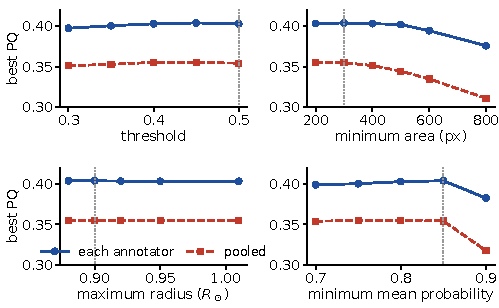
\includegraphics[width=\columnwidth]{figures/sensitivity.pdf}
\caption{Best OOF PQ (707 images, before joining) for each value of one post-processing setting, the others free.}
\label{fig:sens}
\end{figure}

\begin{figure*}[t]
\centering
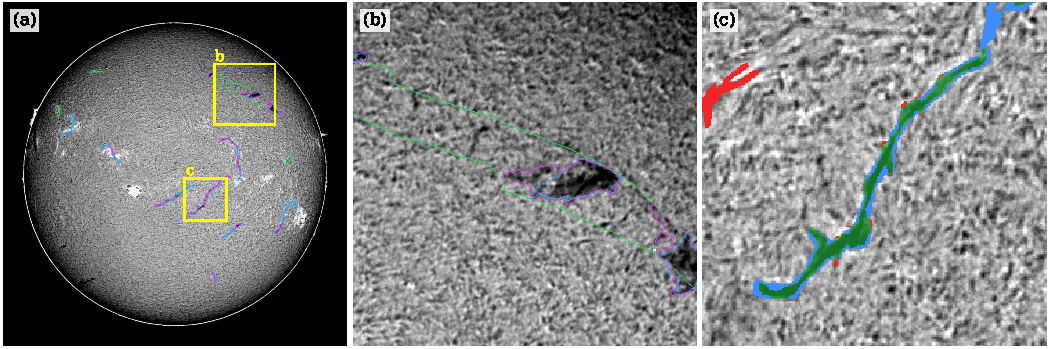
\includegraphics[width=\textwidth]{figures/qualitative.pdf}
\caption{Out-of-fold prediction on fold-0 image 20160204133734Ch, labelled by two annotators (green, blue); model in
magenta. (a) Full disk; boxes mark the zooms. (b) Annotator~1 outlines a large faint region that annotator~2 and the
model restrict to its dark core. (c) Pixel comparison with annotator~1 along one filament: both (green), annotator~1
only (red), model only (blue).}
\label{fig:qual}
\end{figure*}

\begin{figure*}[t]
\centering
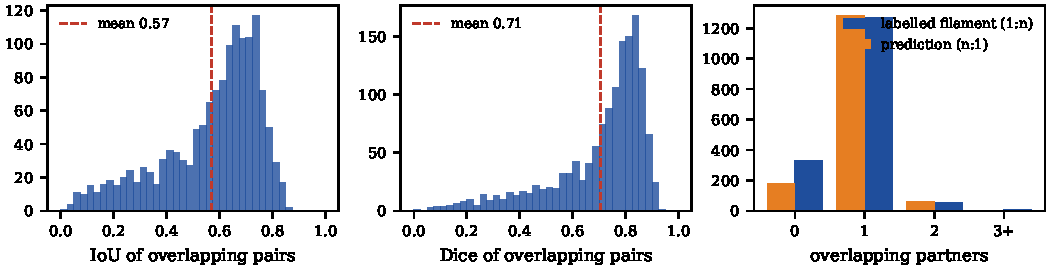
\includegraphics[width=0.9\textwidth]{figures/distributions_fold0.pdf}
\caption{Fold~0 (142 images), final settings: IoU and Dice of every overlapping (label, prediction) pair, and
how many predictions each labelled filament overlaps (1:n) and vice versa (n:1).}
\label{fig:dist}
\end{figure*}

\begin{table}[t]
\centering\small
\caption{Ablations on fold 0 (142 images), PQ against each annotator; the reference is our ResNet34
model with the final settings (0.426); costs are relative to it.}
\label{tab:abl}
\begin{tabular}{@{}lcc@{}}
\toprule
Variant & PQ & train / infer \\
\midrule
ResNet34, whole 1024\,px images (ref.) & 0.426 & 1 / 1 \\
ResNet34, 768\,px crops & 0.420 & 0.6 / 1 \\
ResNet50, 768\,px crops & 0.426 & 1.0 / 1.7 \\
Average of ResNet34 and ResNet50 & 0.430 & 2.0 / 2.7 \\
Learned keep/drop score per filament$^a$ & +0.004 & \\
Thresholds re-matched for averaged maps & $\le$+0.003 & \\
\bottomrule
\end{tabular}\\[2pt]
{\footnotesize $^a$gradient-boosted trees on 23 shape, probability and position features, cross-validated
by image; no gain under pooled scoring.}
\end{table}

\subsection{Ablations}
Table~\ref{tab:abl} varies one component at a time. A ResNet50 encoder needs crops to fit two 16\,GB GPUs and
only recovers the ResNet34 result at about 1.7 times the training and inference cost of the cropped ResNet34;
averaging two architectures gains 0.004 at two to three times the cost. A learned per-filament score that replaces the two
filters gains 0.004, and re-matching the confidence threshold for averaged maps at most 0.003. We kept the
simpler, cheaper configuration.
\subsection{Efficiency}
Training takes about 70\,min per fold on two T4 GPUs. Inference costs about 0.8\,s per image and model with
test-time augmentation (about 4\,s for the five-model ensemble) plus 0.2\,s of single-core post-processing.

\section{Analysis}
\subsection{Scoring rule}
Pooled PQ is not just lower: it depends on how many people labelled an image. On fold 0, PQ against each
annotator is the same for images with one, two and three annotators (0.425, 0.430, 0.425), while pooled PQ
falls (0.425, 0.350, 0.292), because a filament drawn by three annotators appears three times in the pooled
list and a non-overlapping prediction can match only one copy. The public leaderboard's level (0.35--0.36)
is consistent with our pooled OOF estimate (0.353) rather than with the per-annotator one (0.408), a gap
four times the leaderboard's sampling noise on about 90 images (s.d.\ 0.012). Re-tuning for the pooled rule
keeps slightly more filaments (6.8 instead of 6.6 per image on fold~0) and gains 0.003, below what the
public leaderboard can resolve.
\subsection{Where the error remains}
For matched pairs on fold 0, 53\% of missed labelled pixels lie in the outer 2\,px of a filament's body and
61\% of extra predicted pixels lie within 2\,px outside the label: boundary placement, where annotators also
disagree, dominates (Fig.~\ref{fig:qual}c). Thin structures narrower than 5\,px (barbs and threads) are only
2.4\% of the labelled area; within correctly detected filaments the model captures 45\% of them versus 81\% of
other filament pixels, and capturing all of them would raise SQ by at most 0.016. The missed barbs are
essentially absent from the probability map (median probability 0.008, the same as unlabelled pixels beside
the filament). We therefore tried an image-guided refinement that re-decides a thin band around each
predicted filament by local darkness (contrast to a morphological closing of the image) and lets filaments
grow through connected dark pixels. Tuned on half of fold~0, it raised the share of all labelled thin parts
covered from 35.5\% to at most 40.3\% while PQ changed by $-0.007$ to $+0.001$ (held-out half: $-0.001$):
at this contrast, annotated barbs are not separable from the surrounding chromospheric fibrils, and we did not
adopt it.
\subsection{Limitations}
All numbers come from one architecture family; thresholds were tuned on the same OOF predictions they are
evaluated on, so the OOF score is slightly optimistic; and the leaderboard's exact rule for
multiply-annotated test images is inferred, not documented.

\section{Conclusion}
Treating annotator disagreement as the central property of the data led to soft targets, PQ-based model
selection and PQ-tuned post-processing. The resulting pipeline exceeds human agreement out of fold at modest
cost, and our ablations suggest that further gains will come from better handling of label noise and
boundaries rather than from larger models. Code: \url{https://github.com/Mapalo90/competition}.

\balance
{\footnotesize
\begin{thebibliography}{9}
\setlength{\itemsep}{0pt}
\bibitem{magfilo} A.~Ahmadzadeh \emph{et al.}, ``A dataset of manually annotated filaments from H-alpha
observations,'' \emph{Scientific Data}, vol.~11, p.~1031, 2024.
\bibitem{kirillov2019} A.~Kirillov, K.~He, R.~Girshick, C.~Rother, and P.~Doll\'ar, ``Panoptic segmentation,''
in \emph{Proc.\ CVPR}, 2019, pp.~9404--9413.
\bibitem{unet} O.~Ronneberger, P.~Fischer, and T.~Brox, ``U-Net: Convolutional networks for biomedical image
segmentation,'' in \emph{Proc.\ MICCAI}, 2015, pp.~234--241.
\bibitem{resnet} K.~He, X.~Zhang, S.~Ren, and J.~Sun, ``Deep residual learning for image recognition,'' in
\emph{Proc.\ CVPR}, 2016, pp.~770--778.
\bibitem{smp} P.~Iakubovskii, ``Segmentation Models Pytorch,'' GitHub repository, 2019.
\bibitem{vnet} F.~Milletari, N.~Navab, and S.-A.~Ahmadi, ``V-Net: Fully convolutional neural networks for
volumetric medical image segmentation,'' in \emph{Proc.\ 3DV}, 2016, pp.~565--571.
\bibitem{adamw} I.~Loshchilov and F.~Hutter, ``Decoupled weight decay regularization,'' in \emph{Proc.\ ICLR},
2019.
\end{thebibliography}}
\end{document}
